
\begin{figure}[H]
    \begin{center}
        
\includegraphics[width=5cm]{../content/images/Trello/TrelloLogo.png}
        \caption{TRELLO Logo}
    \end{center}
\end{figure}

Trello ist ein Online-Tool zum verwalten von Aufgaben und gehört dem Unternehmen Atlassan. 
Das beliebte Online-Tool ist seit 2011 auf dem Markt und erfeut sich an milionen von Benutzern.


%------------------------------------------------------- 
%TRELLO BOARD SCREENSHOT
\begin{figure}[H]
    \begin{center}
        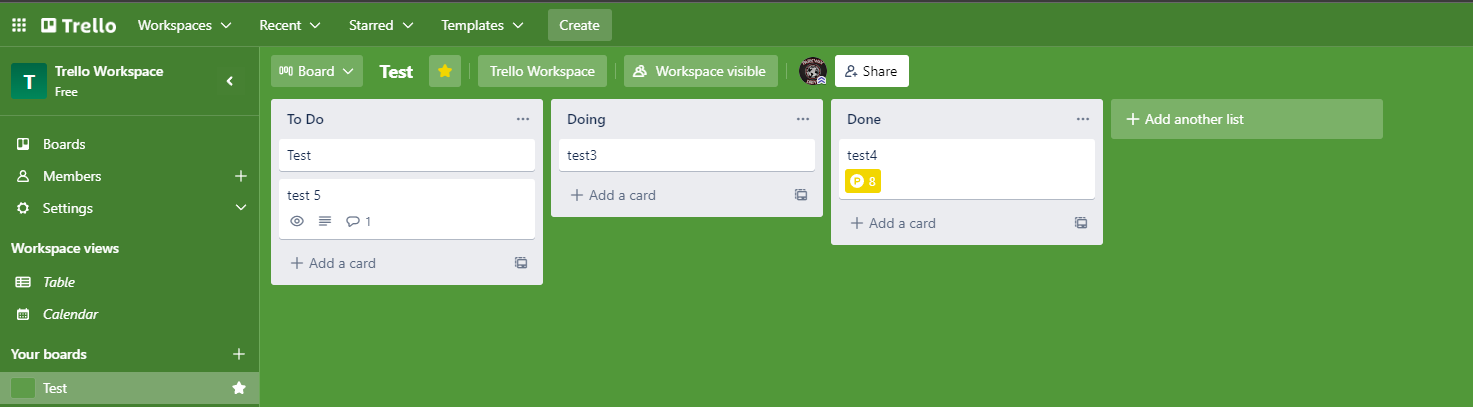
\includegraphics[width=16cm]{../content/images/Trello/TrelloBoard.png}
        \caption{TRELLO board}
    \end{center}
\end{figure}
%------------------------------------------------------- 

Das Layout entspricht einem klassischen Kanban-Board, welches jedoch nach belieben angepasst und
modifiziert werden kann. Das geschäftsmodell von trello lässt sich am ehsten als ''freemium'' bezeichen, die nötigsten Funktionen
sind gratis, reicht dies nicht aus, so kann ein Premium-Abo für 10.- pro monat abgeschlossen werden.
Beim Testen des Dienstes ist mir das penetrante anbieten des 30Days-Free-Trial angebotes, welche sich nach abschluss der 30 Tage automatisch verlängert
besonders negativ aufgefallen.\\
\space
%------------------------------------------------------- 
%TRELLO CARD SCREENSHOT WRAPPER
\begin{figure}[H]
    \begin{center}
        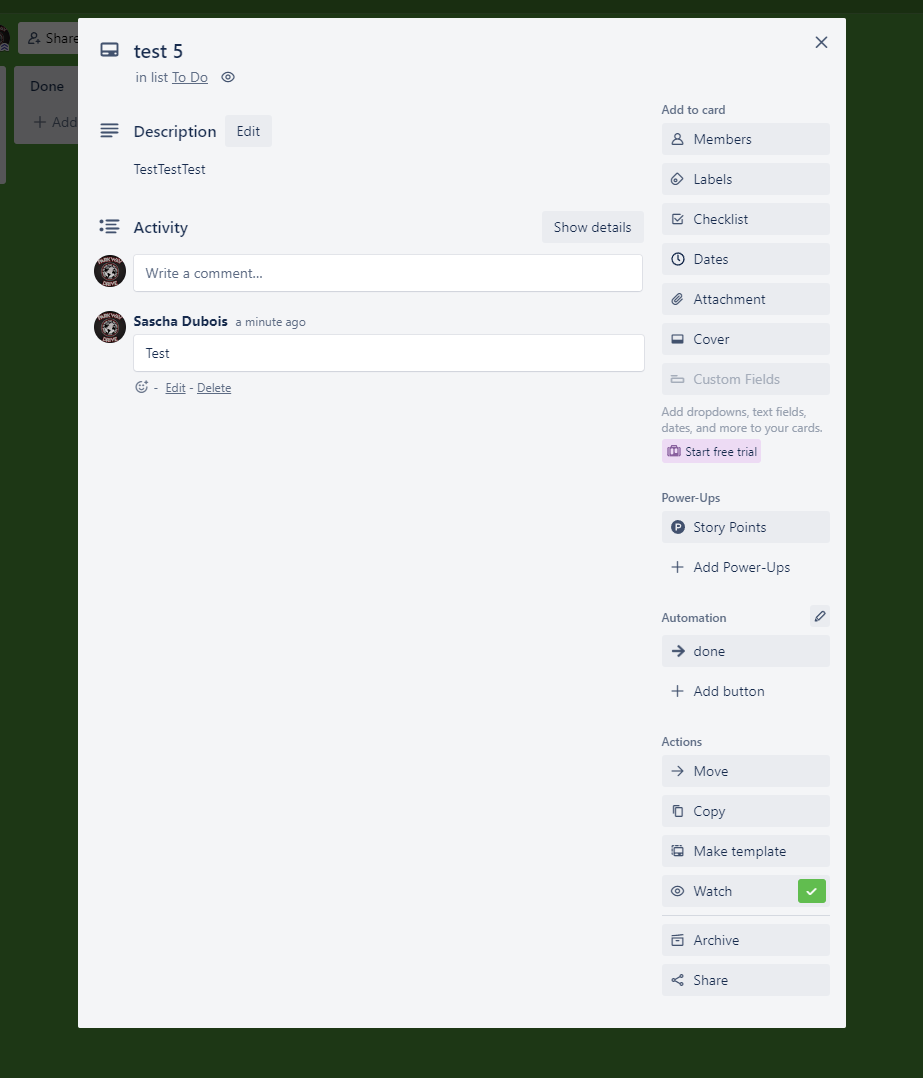
\includegraphics[width=5cm]{../content/images/Trello/TrelloCard.png}
        \caption{TRELLO Card}
    \end{center}
\end{figure}
%------------------------------------------------------- 

Dem Trello-Board können sogenannte ''Cards'' hinzugefügt werden. Den ''Cards'' kann man standartmässig
einen Titel, eine Beschreibung und Kommentare hinzufügen. Es lassen sich ausserdem
Personen, Labels, Checklists, Covers und Anhänge anfügen.\\
Fängt man das erste Projekt mit Trello an, so scheinen die Funktionen relativ übersichtlich zu sein.
Die grösste stärke, meiner Meinung nach, liegt jedoch in der konfigurierbarkeit von Trello. Es können nähmlich
''PowerUps'' eingefügt werden. PowerUps sind Plugins, mit denen die Funktionen von Trello beliebig erweitert werden können.
Zum Beispiel gibt es standartmässig keine möglichkeit den Cards irgendpwelche StoryPoints oder Stunden zuzuweisen.
Fügt man jedoch das entsprechende PowerUp hinzu so ist dies kein Problem mehr.\\
Und es gibt fast für alles ein entsprechendes PowerUp, so können auch Excel-Daten mittels PowerUp importiert werden.
Dem Benutzer sind also nur wehnig Grenzen gesetzt, was die Personalisierung von Trello angeht.\\

%------------------------------------------------------- 
%TRELLO POWERUPS SCREENSHOT WRAPPER
\begin{figure}[H]
    \begin{center}
        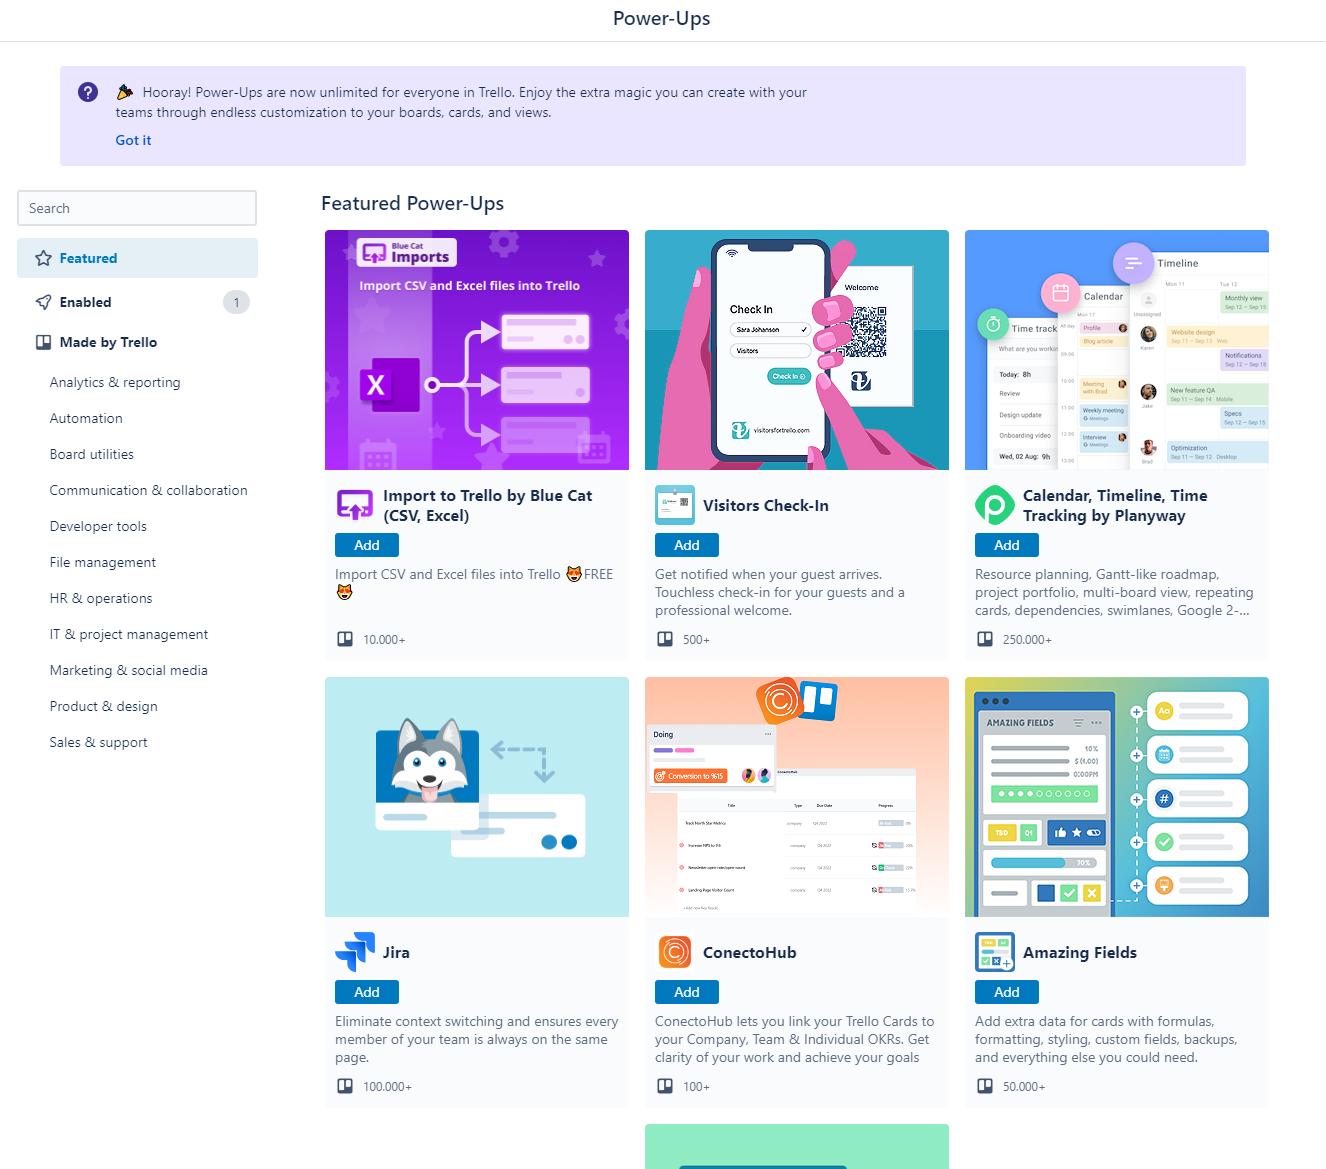
\includegraphics[width=8cm]{../content/images/Trello/PowerUps.png}
        \caption{TRELLO PowerUps}
    \end{center}
\end{figure}
%------------------------------------------------------- 

PowerUps können in einer art App-Store durchsucht und hinzugefügt werden.\\
Da die PowerUps auch von Trello-Usern erstellt werden können, gibt es fast für jeden Use-Case ein entsprechendes PowerUp.
 
%------------------------------------------------------- 
%TRELLO DETAILS TABLE
\begin{table}[H]
    \centering
    \settowidth\tymin{executeIncomingCommand()}
    \setlength\extrarowheight{2pt}
    \begin{tabulary}{1.0\textwidth}{|L|L|}
      \hline
      \textbf{Besitzer} &
      Atlassan\\
      \hline
      \textbf{Gründung} &
      2011\\
      \hline
      \textbf{Plattform} &
      Web\\
      \hline
      \textbf{Layout} &
      Kanban\\
      \hline
      \textbf{Geschäftsmodell} &
      Freemium\\
      \hline
    \end{tabulary}
    \caption{TRELLO Details}
  \end{table}
%------------------------------------------------------- 

%------------------------------------------------------- 
%TRELLO RATING TABLE
\begin{table}[H]
    \centering
    \settowidth\tymin{executeIncomingCommand()}
    \setlength\extrarowheight{2pt}
    \begin{tabulary}{1.0\textwidth}{|L|L|L|}
      \hline
      \textbf{Bewertungspunkt} &
      \textbf{Bewertung} &
      \textbf{Begründung} \\
      \hline
      \textbf{Benutzerfreundlichkeit} &
      ****&
      Die Hohe konfigurierbarkeit führt zwangsläufig dazu, dass die Übersichtlichkeit der Funktionen etwas leidet\\
      \hline
      \textbf{Darstellung} &
      *****&
      Klassisches Kanbanboard, Backgrounds und Design können nach belieben angepasst werden\\
      \hline
      \textbf{Usability} &
      *****&
      Da Trello eine Webapplikation ist, ist sie auf allen webfähigen Geräten zugänglich\\
      \hline
      \textbf{Funktionalität} &
      *****&
      Durch die PowerUps kann die Funktionalität nach belieben erweitert werden\\
      \hline
      \textbf{Preis} &
      ****&
      Die Gratisversion ist absolut ausreichend, jedoch wird man immer wieder dazu gedrängt ein Premium-Abo abzuschliessen welches nicht gerade günstig ist\\
      \hline
    \end{tabulary}
    \caption{TRELLO Bewertung}
  \end{table}
%------------------------------------------------------- 
\space
\textbf{Punkte zur berücksichtigung in eigenem Projekt:}
\begin{itemize}
    \item Konfigurierbarkeit mittels anfügbarer Komponenten (PowerUps)
    \item Kanban Layout
    \item Design
\end{itemize}

  
  